% Meta-Informationen -------------------------------------------------------
%		Informationen über das Dokument, wie z.B. Titel, Autor, Matrikelnr. etc
%		werden in der Datei _Meta.tex definiert und können danach global
%		verwendet werden.
% --------------------------------------------------------------------------
% Informationen ------------------------------------------------------------
% 	Definition von globalen Parametern, die im gesamten Dokument verwendet
% 	werden können (z.B auf dem Deckblatt etc.).
% --------------------------------------------------------------------------
\newcommand{\titel}{End-to-End Reinforcement Learning Training of a Convolutional Neural Network to achieve an autonomous driving agent resilient to light changes}
\newcommand{\art}{Master's Thesis}
\newcommand{\ort}{Leipzig}
\newcommand{\hochschule}{Universität Leipzig}
\newcommand{\fachgebiet}{Database Department}
\newcommand{\fakultaet}{Faculty of Mathematics and Computer Science}
\newcommand{\institut}{Institute of Computer Science}
\newcommand{\autor}{Georg Schneeberger}
\newcommand{\matrikelnr}{3707914}
\newcommand{\erstbetreuer}{Prof. Dr. Erhard Rahm}
\newcommand{\zweitbetreuer}{Dr. Thomas Burghardt}
\newcommand{\drittbetreuer}{Martin Lorenz}
\newcommand{\jahr}{2024}
\newcommand{\invnr}{1337}
\newcommand{\eingereicht}{28.06.2024}

% Eigene Befehle
\newcommand{\todo}[1]{\textbf{\textsc{\textcolor{red}{(TODO: #1)}}}}

% Autorennamen in small caps
\newcommand{\AutorZ}[1]{\textsc{#1}}
\newcommand{\Autor}[1]{\AutorZ{\citeauthor{#1}}}

% Befehle zur semantischen Auszeichnung von Text
\newcommand{\NeuerBegriff}[1]{\textbf{#1}}
\newcommand{\Fachbegriff}[1]{\textit{#1}}
\newcommand{\Prozess}[1]{\textit{#1}}
\newcommand{\Webservice}[1]{\textit{#1}}
\newcommand{\Eingabe}[1]{\texttt{#1}}
\newcommand{\Code}[1]{\texttt{#1}}
\newcommand{\Datei}[1]{\texttt{#1}}
\newcommand{\Datentyp}[1]{\textsf{#1}}
\newcommand{\XMLElement}[1]{\textsf{#1}}

% Abkürzungen
\newcommand{\vgl}{Vgl.\ }
\newcommand{\ua}{\mbox{u.\,a.\ }}
\newcommand{\zB}{\mbox{z.\,B.\ }}
\newcommand{\bs}{$\backslash$}

% Einfache Anführungszeichen in texttt
\newcommand{\sq}{\textquotesingle}



% Dokumentenkopf -----------------------------------------------------------
% 	Diese Vorlage basiert auf "scrreprt" aus dem koma-script.
%		Die Option draft sollte beim fertigen Dokument ausgeschaltet werden.
% --------------------------------------------------------------------------
\documentclass[
	11pt,					% Schriftgröße
	DIV=10,
	ngerman,				% für Umlaute, Silbentrennung etc.
	a4paper,				% Papierformat
	oneside,				% einseitiges Dokument
	titlepage,				% es wird eine Titelseite verwendet
	parskip=half,			% Abstand zwischen Absätzen (halbe Zeile)
	headings=normal, % Größe der Überschriften verkleinern
	numbers=withendperiod, % Fügt in den Überschriften nach den Zahlen einen Punkt ein
	listof=totoc,				% Verzeichnisse im Inhaltsverzeichnis aufführen
	bibliography=totoc,				% Literaturverzeichnis im Inhaltsverzeichnis aufführen
	index=totoc,				% Index im Inhaltsverzeichnis aufführen
	captions=tableheading,		% Beschriftung von Tabellen oberhalb ausgeben
	final					% Status des Dokuments (final/draft)
]{scrreprt}

\renewcommand*\chapterheadstartvskip{\vspace*{-1.0cm}}

% Bentigte Packages -------------------------------------------------------
%		Weitere Packages, die benötigt werden, sind in die Datei Packages.tex
%		"ausgelagert", um die Vorlage möglichst übersichtlich zu halten.
% --------------------------------------------------------------------------
% Anpassung des Seitenlayouts ----------------------------------------------
% 	siehe Seitenstil.tex
% --------------------------------------------------------------------------
\usepackage[
	automark,			% Kapitelangaben in Kopfzeile automatisch erstellen
	headsepline,	% Trennlinie unter Kopfzeile
	ilines				% Trennlinie linksbündig ausrichten
]{scrlayer-scrpage}
\usepackage{scrhack} % Disable some warnings

\usepackage{pseudocode}
\usepackage{nicefrac}

% Für eine schöne Anordnung von Bildern
\usepackage{subfigure}

\usepackage{dsfont}
%\usepackage{color}
%
%% Define user colors using the RGB model
%\definecolor{yellow}{rgb}{0.0,1.0,0.0}
%\definecolor{rot}{rgb}{1.0,0.0,0.0}

% Anpassung an Landessprache -----------------------------------------------
% 	Verwendet globale Option german siehe \documentclass
% --------------------------------------------------------------------------
\usepackage[ngerman]{babel}

% Umlaute ------------------------------------------------------------------
% 		Umlaute/Sonderzeichen wie äöüß direkt im Quelltext verwenden (CodePage).
%		Erlaubt automatische Trennung von Worten mit Umlauten.
% --------------------------------------------------------------------------
\usepackage[utf8]{inputenc}
\usepackage[T1]{fontenc}
%\usepackage{ae} % "schöneres" ä
\usepackage{textcomp} % Euro-Zeichen etc.
\usepackage{lmodern} % schööön

% Grafiken -----------------------------------------------------------------
% 		Einbinden von Grafiken [draft oder final]
% 		Option [draft] bindet Bilder nicht ein - auch globale Option
% --------------------------------------------------------------------------
\usepackage[dvips,final]{graphicx}
\usepackage{wrapfig}
\graphicspath{{Bilder/}} % Dort liegen die Bilder des Dokuments

% Befehle aus AMSTeX für mathematische Symbole z.B. \boldsymbol \mathbb ----
\usepackage{amsmath,amsfonts,amsthm}

% Für Index-Ausgabe; \printindex -------------------------------------------
\usepackage{makeidx}

% Einfache Definition der Zeilenabstände und Seitenränder etc. -------------
\usepackage{setspace}
\usepackage{geometry}

% für gedrehte Tabellen
\usepackage{rotating} 

% Symbolverzeichnis --------------------------------------------------------
% 	Symbolverzeichnisse bequem erstellen, beruht auf MakeIndex.
% 		makeindex.exe %Name%.nlo -s nomencl.ist -o %Name%.nls
% 	erzeugt dann das Verzeichnis. Dieser Befehl kann z.B. im TeXnicCenter
%		als Postprozessor eingetragen werden, damit er nicht ständig manuell
%		ausgeführt werden muss.
%		Die Definitionen sind ausgegliedert in die Datei Abkuerzungen.tex.
% --------------------------------------------------------------------------
\usepackage[intoc]{nomencl}
  \let\abbrev\nomenclature
  \renewcommand{\nomname}{Abkürzungsverzeichnis}
  \setlength{\nomlabelwidth}{.25\hsize}
  \renewcommand{\nomlabel}[1]{#1 \dotfill}
  \setlength{\nomitemsep}{-\parsep}

% Zum Umfließen von Bildern -------------------------------------------------
\usepackage{floatflt}

% Zum Einbinden von Programmcode --------------------------------------------
\usepackage{listings}
\usepackage{xcolor} 
\definecolor{hellgelb}{rgb}{1,1,0.9}
\definecolor{colKeys}{rgb}{0,0,1}
\definecolor{colIdentifier}{rgb}{0,0,0}
\definecolor{colComments}{rgb}{1,0,0}
\definecolor{colString}{rgb}{0,0.5,0}
\lstset{%
    float=hbp,%
    basicstyle=\texttt\small, %
    identifierstyle=\color{colIdentifier}, %
    keywordstyle=\color{colKeys}, %
    stringstyle=\color{colString}, %
    commentstyle=\color{colComments}, %
    columns=flexible, %
    tabsize=2, %
    frame=single, %
    extendedchars=true, %
    showspaces=false, %
    showstringspaces=false, %
    numbers=left, %
    numberstyle=\tiny, %
    breaklines=true, %
    backgroundcolor=\color{hellgelb}, %
    breakautoindent=true, %
%    captionpos=b%
}

% Lange URLs umbrechen etc. -------------------------------------------------
\usepackage{url}


\usepackage{makecell}

%% Wichtig für korrekte Zitierweise ------------------------------------------

\usepackage[autocite=inline, sorting=none]{biblatex}
\bibliography{quellen} % Name der .bib-Datei

\usepackage{csquotes} % Empfohlen, um Zitierten Text richtig darzustellen

% ermöglicht Zeilenumbrüche in Captions
\usepackage{caption}


% PDF-Optionen --------------------------------------------------------------
\usepackage[
bookmarks,
bookmarksopen=true,
pdftitle={\titel},
pdfauthor={\autor},
pdfcreator={\autor},
pdfsubject={\titel},
pdfkeywords={\titel},
colorlinks=true,
%linkcolor=red, % einfache interne Verknüpfungen
%anchorcolor=black,% Ankertext
%citecolor=blue, % Verweise auf Literaturverzeichniseinträge im Text
%filecolor=magenta, % Verknüpfungen, die lokale Dateien öffnen
%menucolor=red, % Acrobat-Menüpunkte
%urlcolor=cyan, 
% für die Druckversion können die Farben ausgeschaltet werden:
linkcolor=black, % einfache interne Verknüpfungen
anchorcolor=black,% Ankertext
citecolor=black, % Verweise auf Literaturverzeichniseinträge im Text5
filecolor=black, % Verknüpfungen, die lokale Dateien öffnen
menucolor=black, % Acrobat-Menüpunkte
urlcolor=black, 
%backref,
%pagebackref,
plainpages=false,% zur korrekten Erstellung der Bookmarks
pdfpagelabels,% zur korrekten Erstellung der Bookmarks
hypertexnames=false,% zur korrekten Erstellung der Bookmarks
linktocpage % Seitenzahlen anstatt Text im Inhaltsverzeichnis verlinken
]{hyperref}

% Zum fortlaufenden Durchnummerieren der Fußnoten ---------------------------
\usepackage{chngcntr}


% für lange Tabellen
\usepackage{longtable}
\usepackage{array}
\usepackage{ragged2e}
\usepackage{lscape}

\usepackage{supertabular}

% Spaltendefinition rechtsbündig mit definierter Breite ---------------------
\newcolumntype{w}[1]{>{\raggedleft\hspace{0pt}}p{#1}}

% Formatierung von Listen ändern
\usepackage{paralist}
% Standardeinstellungen:
% \setdefaultleftmargin{2.5em}{2.2em}{1.87em}{1.7em}{1em}{1em}

\usepackage{tablefootnote}
% für Ausblenden der Seitenzahl
\usepackage{lipsum}

% Erstellung eines Index und Abkürzungsverzeichnisses aktivieren -----------
\makeindex
% makeindex Masterarbeit.nlo -s nomencl.ist -o Masterarbeit.nls
\makenomenclature


% Kopf- und Fußzeilen, Seitenränder etc. -----------------------------------
% Zeilenabstand ------------------------------------------------------------
\onehalfspacing 
% \setstretch{1,5}

% Seitenränder -------------------------------------------------------------
\geometry{paper=a4paper,left=25mm,right=20mm,top=20mm, bottom=25mm}
% Notfall maße :)
%\geometry{paper=a4paper,left=35mm,right=25mm,top=25mm, bottom=25mm}



% Kopf- und Fußzeilen ------------------------------------------------------
\pagestyle{scrheadings}

% Kopf- und Fußzeile auch auf Kapitelanfangsseiten -------------------------
\renewcommand*{\chapterpagestyle}{scrheadings}

% Schriftform der Kopfzeile ------------------------------------------------
\renewcommand{\headfont}{\normalfont}

% Kopfzeile ----------------------------------------------------------------
\ihead{\textit{\headmark}}
\chead{}
%\ohead{\includegraphics[scale=1]{Bilder/logoKlein.JPG}}
\ohead{}
\setlength{\headheight}{8mm} % Höhe der Kopfzeile
\setheadwidth[0pt]{textwithmarginpar} % Kopfzeile über den Text hinaus verbreitern

% Fußzeile -----------------------------------------------------------------
% \ifoot{\copyright\ \autor \\ \invnr}
% \ifoot{\copyright\ \autor \\ \matrikelnr}
\ifoot{\autor \\ \matrikelnr}
\cfoot{}
\ofoot{\pagemark}
\setlength{\footskip}{12mm}
\setfootwidth[0pt]{text}

% Überschriften ------------------------------------------------------------
\renewcommand*\chapterheadstartvskip{\vspace*{-0.5cm}} % Platz vor einer Überschrift eines neuen Kapitels


% erzeugt ein wenig mehr Platz hinter einem Punkt --------------------------
\frenchspacing

% Schusterjungen und Hurenkinder vermeiden
\clubpenalty = 10000
\widowpenalty = 10000 
\displaywidowpenalty = 10000


% Quellcode-Ausgabe formatieren --------------------------------------------
%\lstset{numbers=left, numberstyle=\tiny, numbersep=5pt, breaklines=true}
%\lstset{emph={square}, emphstyle=\color{red}, emph={[2]root,base}, emphstyle={[2]\color{blue}}}

\definecolor{gray}{rgb}{0.9,0.9,0.9}

\lstset{%
		basicstyle=\small\ttfamily,language={[LaTeX]TeX},
		numbersep=5mm, 
		numbers=left,
		numberstyle=\tiny,
		breaklines=true,
		framexleftmargin=8mm, 
		xleftmargin=8mm,
		backgroundcolor=\color{gray},
		captionpos=b
}%

% Fußnoten fortlaufend durchnummerieren ------------------------------------
\counterwithout{footnote}{chapter}

% Definitionen

\newtheorem{definition}{Definition}


% Eigene Definitionen für Silbentrennung
\hyphenation{Trenn-bar-es}

% Das eigentliche Dokument -------------------------------------------------
%		Der eigentliche Inhalt des Dokuments beginnt hier. Die einzelnen Seiten
%		und Kapitel werden in eigene Dateien ausgelagert und hier nur inkludiert.
% --------------------------------------------------------------------------

\begin{document}
% auch subsubsection nummerieren
\setcounter{secnumdepth}{3}
\setcounter{tocdepth}{3}

% keine Kopf-/Fußzeilen bei Deckblatt und Abstract
\ofoot{}
% Deckblatt
\thispagestyle{plain}
\begin{titlepage}

\begin{center}

\includegraphics[height=7cm]{Bilder/Uni-L.png}\\[2.5ex]

\institut\\
\fakultaet\\
\fachgebiet\\[6ex]

\textbf{\large\titel}\\[1.5ex]
\art\\[6ex]

\normalsize
submitted by:\\
\autor\\[1.5ex]
matriculation number:\\
\matrikelnr\\[1.5ex]
Supervisor:\\
\erstbetreuer\\
\zweitbetreuer\\[1.0ex]
\end{center}

%\begin{tabbing}
%\hspace{3.5cm}\= \kill
%   vorgelegt von: \> \autor\\[1.2ex]
%   Matrikelnummer: \> \matrikelnr\\[1.2ex]
%    \> \\
%   Betreuer: \> \erstbetreuer\\[1.2ex]
%    \> \zweitbetreuer
%\end{tabbing}

\begin{center}
\copyright\ \jahr\\[1.0ex]
\end{center}

\singlespacing
\small
\noindent This thesis and its parts are \textbf{protected by copyright}. Any use outside the narrow limits of copyright law without the consent of the author is prohibited and punishable by law. This applies in particular to reproductions, translations, microfilming as well as storage and processing in electronic systems.

\end{titlepage}


\section*{Abstract}
\label{sec:Abstract}

In my master's thesis I will investigate using neural networks for self driving. The goal is to create an autonomous driving agent that is resilient to changes in light conditions. The agent will employ preprocessing steps and a convolutional neural network to achieve this. The agent will be trained using reinforcement learning in a simulated environment with changing light conditions to help the agent generalize.

The reinforcement learning agent's task is to complete a parcour in a simulated environment without collisions. The thesis builds upon previous student's work at the ScaDS.AI \autocite{maximilian}, the task specifications and evaluation approaches are reused for comparability. This thesis focusses on improving the resiliency to changing light conditions.

% TODO ScaDS.AI ist die Schreibweise, wird sie auch im Text so verwendet?


% \section*{Danksagung}
\label{sec:Danksagung}
Danksagung
\newpage
\ofoot{\pagemark}

% Seitennummerierung -------------------------------------------------------
%		Vor dem Hauptteil werden die Seiten in großen römischen Ziffern 
%		nummeriert...
% --------------------------------------------------------------------------
\pagenumbering{Roman}

\tableofcontents			% Inhaltsverzeichnis

% Abkürzungsverzeichnis ----------------------------------------------------
%\input{Inhalt/Glossar}
%\printnomenclature
%\label{sec:Glossar}

%\renewcommand{\lstlistlistingname}{Verzeichnis der Listings}
%\lstlistoflistings	

% ...danach in normalen arabischen Ziffern ---------------------------------
\clearpage
\pagenumbering{arabic}


% Inhalt -------------------------------------------------------------------
%		Hier können jetzt die einzelnen Kapitel inkludiert werden. Sie müssen
%		in den entsprechenden .TEX-Dateien vorliegen. Die Dateinamen können
% 		natürlich angepasst werden.
% --------------------------------------------------------------------------
\chapter{Motivation}
\label{cha:Motivation}

The increasing utilization of artificial intelligence in academia and industry have lead to massive efficiency improvements for all kinds of tasks. The development of autonomous vehicles promises to greatly reduce the number of traffic accidents and transportation cost \autocite{mckinsey}. As a result, researchers and private enterprises from all over the globe are making progress towards fully autonomous driving agents and integrating them in commercial vehicles, many companies started to integrate adaptive cruise control and lane centering assistance \autocite{carreviews}. Due to the recent developments in artificial intelligence and the very high complexity of the task of autonomous driving, artificial intelligence often plays a big role in these systems \autocite{drl_for_ad}.


Predictions for the future of autonomous driving have been very optimistic and although huge progress has been made, the task of fully autonomous driving is still far from being solved \autocite{state_of_autonomous_driving2023}. This thesis aims at contributing to the research in this field by applying reinforcement learning to autonomous driving agents in a simulated environment. This work builds upon the work of \autocite{maximilian} and will use the same task and evaluation metrics. This thesis focusses on improving the agent's resiliency to changing light conditions by training a convolutional neural network end-to-end using reinforcement learning.



%\include{Inhalt/Grundlagen...}

% Literaturverzeichnis -----------------------------------------------------
%		Das Literaturverzeichnis wird aus der Datenbank erstellt.
%		Die genaue Verwendung von biblatex wird hier jedoch nicht erklärt.
%		Links: 	https://ctan.org/pkg/biblatex?lang=de
%						https://de.overleaf.com/learn/latex/Articles/Getting_started_with_BibLaTeX
% --------------------------------------------------------------------------

%{\let\clearpage\relax \chapter{Central Tasks and Research Goals}}


%{\let\clearpage\relax \chapter{Central Tasks and Research Goals2}}

\chapter{Research Goals}
\label{cha:Research Goals}
%\lipsum \autocite{DBLP:books/sp/HarderR01}

The goal of this thesis is to contribute in the domain of autonomous driving by investigating the efficiency and contributions of different implementation details using reinforcement learning in a simulated environment. The thesis will build on the work of \autocite{maximilian} and review the utilised algorithms and implementation details. Implementation changes will be proposed based on research in the field of reinforcement learning and autonomous driving. The contributions of these implementation details will be evaluated on their own and in combination with each other. 

The self driving agent is trained and evaluated on a simulated parcour. Different parcours, lighting settings and motor-power settings are used to evaluate the agent's reliability and generalisation capabilities. The evaluation scenarios will consist of the ones employed by \autocite{maximilian} and potentially additional ones based on related work and the investigated implementation changes.

The task of driving through the parcour is motivated in part by the Scads.AI research facility, it would be ideal to be able to transfer the agent from this thesis to a physical arena at the Scads.AI research facility. The Scads.AI premises are often used for exhibitions and events where a physical self driving agent could be used to raise interest in applications of AI and research. %TODO move this to motivation?


Um ehrlich zu sein war es schwierig diese Paragraphen zu schreiben. Es war schwierig Research Goals zu formulieren, die unterschiedlich von den vorherigen sind.




%{\let\clearpage\relax \chapter{Related Work}}
\chapter{Related Work}
\label{cha:Related Work}

Since this thesis will employ reinforcement learning in the training of the autonomous driving agent it is important to review the current state of the art in reinforcement learning and autonomous driving. Some techniques of the researched works might not be applicable in this thesis due to the smaller scope and availible resources of this thesis, it is still important to review them to understand the current state of the art and to be able to utilise aspects of them. Simulation environments for reinforcement learning and self driving will also be reviewed, since they play a bit role in the state of the art of both fields and will be employed in this thesis.
Finally, some papers about the use of reinforcement learning for self driving will be reviewed.


\section{Reinforcement Learning}

Reinforcement Learning algorithms have been around for a long time, but only recently have they been able to achieve superhuman performance in games and control tasks. Most reinforcement learning algorithm formalize the problem using a state space and an action space and a reward function associated with state transitions. The RL algorithms are built to select an action in a given state and try to maximize the cumulative reward along the state transitions. This process of selecting an action is called the policy.

The classical version of the Q-learning RL algorithm keeps a table of state-action pairs and their associated quality values which are learned/computed during training. These Q-values are used by the algorithms' policy. The amount of state-action pairs can be very large and not feasible to compute in many cases, especially for environments with continuous state and action spaces. %An example of a continuous state space would be the position of an object in a continuous 2D space. 

To solve this problem neural networks have been used to approximate the Q-values, they take a representation of a state from the state space as input. This approach is called Deep Q-Learning, convolutional neural networks are often used \autocite{atari}. The initial success of Deep Q-Learning has led to many improvements and variations of the algorithm, since then RL algorithms have proved to be very useful in a wide range of applications.


A mayor weakness of the initial Deep Q-learning algorithm was its stability during training, the parameter updates of the Q-learning agent's neural network can result in a collapse in performance. Proximal Policy Optimization (PPO) and other algorithms have been developed to improve the training process stability. The PPO \autocite{ppo} algorithm restricts the size of policy changes caused by parameter updates, this ensures the policy cannot change drastically and improves stability. PPO is currently one of the most popular algorithms for reinforcement learning and has already been successfully used in the domain of autonomous driving \autocite{maximilian}.
% other algorithms with better training stability are Double DQN, TRPO
% maybe introduce TRPO as it was the predecessor of PPO


Another major improvement in the domain of reinforcement learning was the combination of neural networks with traditional planning and search algorithms, the most famous example for this is AlphaGo \autocite{alphago}. The search algorithms (typically Monte Carlo Tree Search) evaluate the possible actions at a given state. The neural networks are used for the evaluation of states and actions in the search algorithms. AlphaGo was developed for a 2 player deterministic game with a discrete state and action space. Since then the combination of neural networks and search algorithms has also been used for all kinds of problems, for example single player continuous state and action spaces \autocite{alphagoimprovementmuzero}.


\subsection*{Convolutional Neural Network for Reinforcement Learning}

As mentioned already convolutional neural network are often used in Reinforcement Learning. Convolutional neural networks are a neural network architecture specifically developed for processing image data, they consist of a number of filters and a fully connected neural network. The filters are applied to the image in a sliding window fashion, the filters detect pattern in the image such as for example edges and corners. The fully connected neural network analyses the results of the filters and makes the final prediction.
CNNs are ideal for the use in Reinforcement Learning since Reinforcement Learning problems often require an agent to process visual input. Furthermore CNNs can be trained end-to-end in Reinforcement Learning compared to other feature extraction methods, this means the CNN can learn what features are important for the task at hand.
CNNs typically do not take the raw camera/simulation images but rather preprocessed images, e.g. greyscaled images. Preprocessing steps are discussed in the Methods section \ref*{light_setting_robustness}. Furthermore data augmentation can be done during training, this is another kind of preprocessing. Data augmentation generates new samples from already collected ones by applying transformations to the samples, this can be used to increase the size of the training set and to make the agent more robust.

\section{Self Driving}

As mentioned before there has been a lot of progress in the domain of self driving in recent years, often driven by private enterprises that might not publish their findings in academic journals. Sophisticated self driving algorithms often consist of many components to achieve satisfying performance, Tesla FSD for example uses separate object detection, occupancy and planning components \autocite{teslaEndToEnd}.
This thesis builds directly upon the work of \autocite{jonas_koenig}, \autocite{merlin_flach} and \autocite{maximilian}. \autocite{jonas_koenig} built a self driving agent that was trained to avoid collisions in a simulated arena using an evolutionary approach to neural network training, the agent used visual inputs that were preprocessed before feeding it to the neural network. \autocite{merlin_flach} investigated the feasibility of transferring the agent to the real world, this research showcased many difficulties, most notably the object recognition part of the agent. \autocite{maximilian} investigated a different task than the two previous papers, the agent was trained to pass a parcour by driving through a sequence of goals. This task is identical to the one investigated here. \autocite{maximilian} successfully used PPO to train the agent which was fed preprocessed data similar to \autocite{jonas_koenig}.

Another interesting approach to building self driving agents is using imitation learning \autocite{imitation_learning}, imitation learning agents learn to mimic the behaviour exhibited in the training set. The training set is usually generated by humans driving the car, this approach is rumored to be used by Tesla to train their self driving agents \autocite{teslaEndToEnd}.


% \autocite{autonomous_vehicles_review} %TODO read this paper and cite it

% https://safe-intelligence.fraunhofer.de/en/autonomous-driving

% Papers that use Carla



% Mention experiments from PopCulture/YouTube


\section{Simulation for Reinforcement Learning (and Self Driving)}

Simulations play a huge role in reinforcement learning and the development of self driving agents. Simulations provide a number of benefits over real world experiments. They are much cheaper and faster to run than real world experiments, furthermore they can be run in parallel. In addition the programmers have direct and perfect control over the environment. This allows for much faster experimentation and training of reinforcement learning agents. Simulations also allow for the creation of scenarios that are not possible in the real world, this is especially useful for reinforcement learning agents that are trained to avoid collisions. Simulations also allow for the creation of ground truths, which are often not available in the real world such as perfect sensor data and object bounding boxes. Ground truths are used to evaluate the performance of the agent and can be used to train the agent. In addition the physics of the simulation can be modified, for example it is possible to increase the simulation speed.

Simulated environments, especially games have served as baselines for reinforcement learning algorithms. The most famous baseline are the atari games \autocite{atari}. The need for easy use of reinforcement learning algorithms has led to the development and adoption of the Gynasium API \autocite{gymnasium}, the Gymnasium API defines an interface that can be used to model tasks as reinforcement learning problems. This interface is called a Gym environment, an allows for easy testing of reinforcement learning algorithms on a wide range of tasks. Furthermore the Gymnasium API allows for easy comparison of different algorithms on the same task. A wide range of reinforcement learning frameworks support the Gymnasium API, for example Google's dopamine \autocite{dopamine} and OpenAI's baselines \autocite{sb3}.

Wrappers for Gymnasium environments are often used to facilitate the use of more advanced simulations for environments, such as for example the game engines Unity and Unreal or the physics simulator MuJoCo \autocite{mujoco}. The complexity and interest in self driving has also led to the development of dedicated simulators, such as the Carla \autocite{carla} and the AirSim \autocite{airsim} simulator. The Carla simulator provides researchers with useful features such as weather control and ground truths for object detection and segmentation.

There are also dedicated frameworks for reinforcement learning that directly integrate with game engines, such as the ML-Agents framework \autocite{mlagents} for Unity.\autocite{maximilian} used this framework to train the self driving agent.

% TODO check Ray: https://docs.ray.io/en/latest/rllib/index.html
% TODO check dopamine https://github.com/google/dopamine


\section{Reinforcement Learning for Self Driving}

\autocite{drl_for_ad} review the use of reinforcement learning for autonomous driving, they also describe many improvements for reinforcement learning algorithms that can improve the training stability and performance, such as for example reward shaping.
In addition to published research papers there have been a lot of experiments, tutorials and demonstrations of self driving agents on YouTube and GitHub. The University of Tübingen published their full lecture series on Self-Driving Cars \autocite{tuebingen}, the series also includes a section on reinforcement learning.

% papers that cite carla: https://scholar.google.de/scholar?cites=660591080772510291&as_sdt=2005&sciodt=0,5&hl=de


% Tübingen: % https://www.youtube.com/watch?v=GYnlqiSqZiU&list=PL05umP7R6ij321zzKXK6XCQXAaaYjQbzr&index=13



% TODO reference papers that use the improvements I propose

% Key Papers in RL: https://spinningup.openai.com



\chapter{Methods}
\label{cha:Methods}



\section{Task Description}

In this section I will be describing the task and the simulation environment as these two aspects are the foundation of this thesis and will not change over the course of the project.
The task is to develop an agent using reinforcement learning that is able to complete a parcour in a simulated environment without collisions. The agent has to traverse the parcour by passing through a number of goals indicated by pairs of either red or blue blocks without collisions. This problem belongs to the class of single player continuous state and action space problems. At each timestep the agent uses a neural network to process an image from the environment and produce two actions. The two actions are the acceleration values of the left and right wheel, these acceleration values are applied to the wheels until a new action is selected.% The timesteps do not have a fixed duration, a new timestep is started as soon as the last one is finished. The amount of timesteps per minute will be measured? This is like FPS?

The task and agent are simulated using the Unity game engine, the game engine handles the rendering of the environment, collisions, agent movement and reward functions.


\begin{figure}
     \centering
     \subfigure[Example image of the agent at the start of a parcour with 3 goals in Unity]{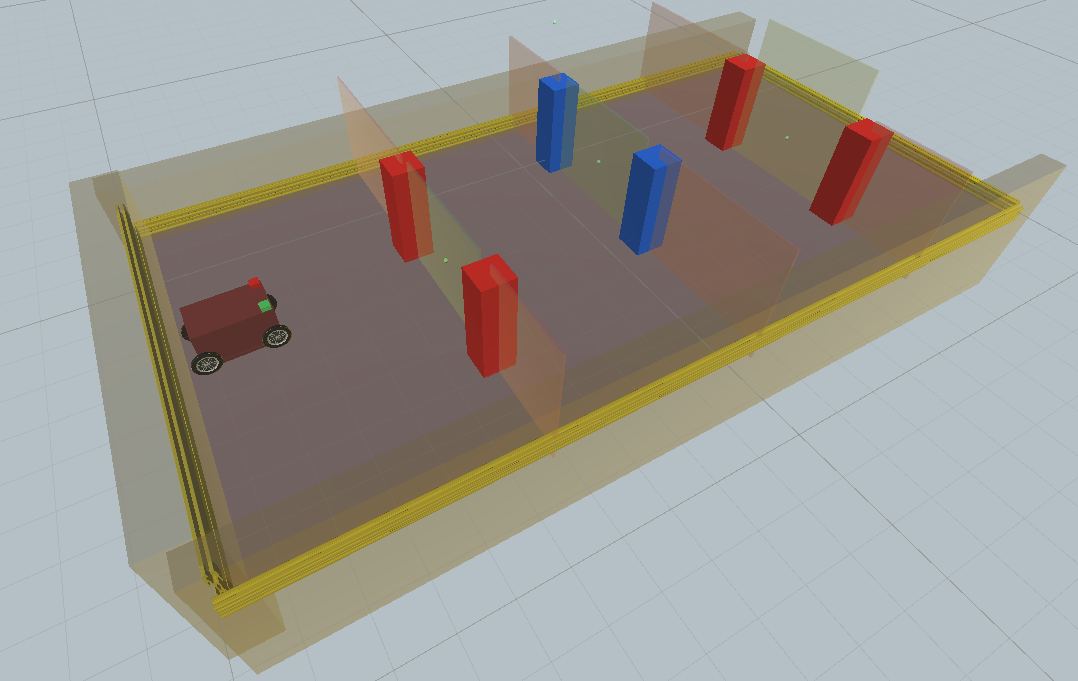
\includegraphics[height=5cm]{Bilder/parcour.png}}\qquad
     \subfigure[Agent camera view]{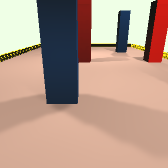
\includegraphics{Bilder/agent_input_image2.png}}\\
     \caption{Unity simulation environment and agent camera view}
\end{figure}


\iffalse
     \begin{figure}[h!]
          \centering
          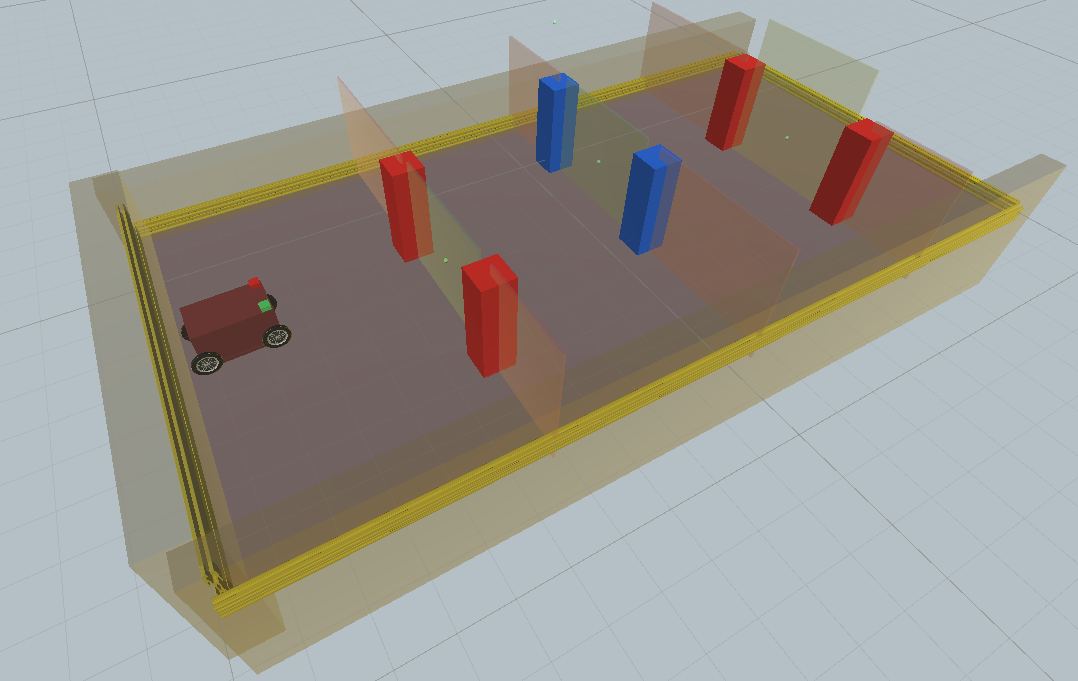
\includegraphics[height=7cm]{Bilder/parcour.png}\\[2.5ex]
          \caption{Example image of the agent at the start of a parcour with 3 goals in Unity}
          \label{task}
     \end{figure}
     \begin{figure}[h!]
          \centering
          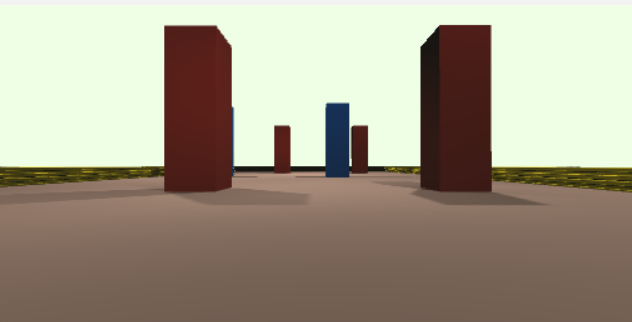
\includegraphics[height=7cm]{Bilder/agent_input_image.png}\\[2.5ex]
          \caption{Example image that will be processed by the agent's convolution neural network.}
          \label{input_image}
     \end{figure}
\fi

% mention the similarity/simplicity of the task


\section{Reinforcement learning algorithm and frameworks}

As outlined in the related works section many different RL algorithms can be used to solve single player continuous state and action space problems. The PPO algorithms is most commonly used for problems of this class and has already been successfully used in the investigated task \autocite{maximilian}. The MuZero \autocite{alphagoimprovementmuzero} could also be used, however this algorithm does require a lot more compute resources during training and inference.
In this thesis the PPO algorithm will be used.

There are multiple approaches to training an agent in the Unity simulation environment as highlighted in the related works section, it is not yet decided which approach will be chosen, therefore I will quickly describe the possible scenarios and highlight their advantages and disavdantages.

\subsection*{Unity and ML-Agents}

Reinforcement learning agents can be trained directly in the Unity simulation environment using the ML-Agents framework \autocite{mlagents}. This approach has the advantage of being very simple to implement and use, since the agent and simulation are in the same framework. The biggest disadvantage of this approach is that it might be difficult to implement some of the implementation details that might be used in this thesis such as the proposed changes for dealing with delayed rewards.
The PPO algorithm by \autocite{mlagents} was used in \autocite{maximilian} to successfully train the agent on the investigated task.

\subsection*{Unity and separate reinforcement learning frameworks}

There are many reinforcement learning frameworks publicly available that can be used to train agents in simulated environments, such as the OpenAI's baselines \autocite{sb3} and Google's dopamine \autocite{dopamine}. These frameworks often support the Gymnasium API \autocite{gymnasium}, wrapping the Unity simulation environment in a Gymnasium environment would allow for easy use of these frameworks. This approach has the advantage of being able to use the many features of these frameworks and makes it easy to change the training algorithms which might be necessary for the investigated implementation details. The disadvantage of this approach is that it might be difficult to wrap the Unity simulation environment in a Gymnasium environment, there already exist frameworks to help with this \autocite{peacefulpie}.


% maybe mention the similarity/simplicity of the task here to show PPO is good


\section{Investigated implementation details}

The goal of this thesis is to answer two questions with a subitem each.
\begin{enumerate}
     \item Is it possible to train an agent to reliably solve the parcours of all difficulty levels?
           \begin{itemize}
                \item Are memory mechanisms necessary in achieving this?
           \end{itemize}
     \item Is it possible to use an end-to-end trained CNN to make the agent robust to changing light conditions?
           \begin{itemize}
                \item Is it possible to use a CNN which is small enough to be used in the JetBot?
           \end{itemize}
\end{enumerate}

\subsection{Improvements for training the agent}

\subsubsection{Reward shaping}

Reward shaping is the practise of providing reinforcement learning agents with frequent and accurate rewards. This helps the agent develop the desired behaviour quicker and more reliably since reward signals are less sparse with reward shaping \autocite{drl_for_ad}. This practice was already employed by \autocite{maximilian} by providing the agent with a reward proportional to its speed, this encourages the agent to drive faster and thus hopefully complete the parcour quicker. This thesis will investigate the use of a reward proportional to the difference in distance to the next goal between timesteps, this should encourage the agent to drive towards the next goal and to drive faster in this direction.


\subsubsection{Dealing with delayed rewards}
Delayed rewards can be a big problem in reinforcement learning and make the training process difficult. Delayed rewards are rewards that are not obtained immediately after the responsible action is taken. In our environment an action \(a_n\) (e.g. turning right) may lead to a collision at state \(s_{n+x}\) which results in a negative reward for action \(a_{n+x}\). The RL algorithm might fail learn to avoid the action \(a_n\).

There are a multiple approaches to dealing with delayed rewards. These approaches use the reward at the current timestep and the near future. These approaches result in a more accurate and dense reward signal and can improve the training stability and performance of the agent.
N-step bootstrapping uses the rewards at the current step and the next \(n\) steps \autocite{nstepbootstrapping}.
A similar approach does not use the reward from the next \(n\) steps but rather the cumulative reward encountered in the next \(n\) seconds \autocite{trackmania}. Due to the continuous nature of the environment this approach might be more suitable than the previous one.


\subsubsection{Time perception}

Two configurations of the agent by \autocite{maximilian} used a memory to enhance the agent's input, the memory consisted of the input of the last few steps of the agent. This technique of stacking the history has been widely used in RL for continuous \autocite{atari} and discrete action spaces \autocite{alphago}. This allows the agent to perceive object movement, time and velocities \autocite{atari}.
In our case the agent needs a history since the next goal could leave the agent's current field of vision.

%However since the investigated environment does not have fixed timesteps this approach might not be as effective. The time elapsed between two steps can vary due to many factors such as varying compute resources. It could prove useful to provide the model with the input of the last few steps and in addition the elapsed time between these steps. % these few sentences only make sense if the varying time is dicussed in the first part of the Methods section

% TODO test other memory mechanisms?
% like for example also feeding the previous time step's hidden layer activation as input
% that way the agent would know the previous "decision" not just the previous input

\subsection{Improvements for Light setting robustness} \label{light_setting_robustness}

\subsubsection{Convolutional Neural Networks}

The works by \autocite{merlin_flach} and \autocite{maximilian} showed that the agent's performance greatly depended on the quality of the input preprocessing pipeline. This object detection pipeline had difficulties detecting objects under varying light settings. This thesis will investigate using convolutional neural networks instead of an object detection pipeline, this should make the agent more robust to varying light settings and improve the performance of the agent.
Using convolutional networks to process images is a common practise in the field of reinforcement learning, due to the ability of these networks to adapt. The convolutional neural network could potentially learn to identify relevant information in images more reliably than the previously used image detection pipeline. The research by \autocite{merlin_flach} showed that not all the information provided by the object detection pipeline was considered to be relevant by the neural network, this could be mitigated by training the CNN end-to-end.
As a starting point for experimentation the CNN architecture will be the same as \autocite{human_level_control}.

% we use the default CnnPolicy network, is it the same as the one described in Atari?
% architecture: https://github.com/DLR-RM/stable-baselines3/blob/d671402c9373391f44d8a2ad11deed615e0f4bae/stable_baselines3/common/torch_layers.py#L89-L106
% it is exactly as described in "Human-level control through deep reinforcement learning"
% \autocite{atari} has a slightly smaller NN

% (more robustness?) (previous input was shit (sim2real paper wegen x, y, width, height input problem)) (previous system higly depended on bounding box detection)


\subsubsection{Feature reduction / preprocessing}

There are several preprocessing approaches that can be used to prepare an image for processing by a convolutional network. The goal of these approaches is to reduce the feature space to increase processing speed, they can also help encourage the network to generalize. The following steps were taken in the foundational \autocite{atari} paper. These techniques will be used due to the similar complexity of our task and many atari games.

\begin{description}
     \item[Downsampling] reduces size of input space
     \item[converting to greyscale] reduces size of input space and potentially removes irrelevant information
     \item[Rescaling pixel values to between 0 and 1] can help the neural network learn quicker % see https://machinelearningmastery.com/how-to-improve-neural-network-stability-and-modeling-performance-with-data-scaling/
\end{description}


\subsubsection{Histogram Equalization}

The previous work this thesis builds upon used the HSV colour space to extract the differently coloured objects. colours in this space consist of three values, one for the hue, saturation and brightness. The hue value was used for extracting the objects. In theory the utilization of this colour space should make the object detection resilient to changes in brightness since this information does not affect the hue value.
Convolutional neural network typically use the RGB colour space or a greyscale colour space. A histogram equalization of the input images could play a big role in making the agent more resilient to changes in illumination, with which the agent by \autocite{maximilian} struggled with. Image d) in \ref{fig:4bildchen} shows the effect of histogram equalization on an image, the image looks worse for identifying objects. This suggests the equalization might not be necessary/useful, it is to be investigated during the implementation/experimentation phase.


%* histogram equalization / enhance contrast (preprocessing) https://stackoverflow.com/questions/39308030/how-do-i-increase-the-contrast-of-an-image-in-python-opencv

% \autocite*{drl_for_ad} shows a lot of best practises in RL for autonomous driving

\begin{figure}
     \centering
     \subfigure[Original Image]{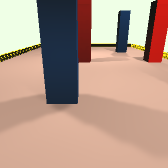
\includegraphics{Bilder/agent_input_image2.png}}\qquad
     \subfigure[Downsampled image]{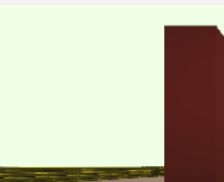
\includegraphics{Bilder/downsampled.png}}\\
     \subfigure[greyscale]{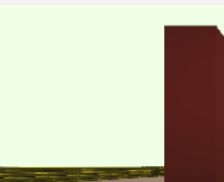
\includegraphics{Bilder/greyscaled.png}}\qquad
     \subfigure[histogram equalized image]{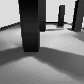
\includegraphics{Bilder/equalized.png}}
     \caption{4 Stages of preprocessing images for the CNN}
     \label{fig:4bildchen}
\end{figure}


\section{Training Process}


\subsection*{Training Parcours}
The PPO Reinforcement Learning algorithm requires the agent to be placed in a simulation environment similar to the evaluation environment to achieve good results. The agent will be placed in an arena with goal objects during training. In previous work \autocite{maximilian} two different training regimes were used, Single-Goal-Training and Full-Map-Training. In Single-Goal-Training the training was stopped after completing the first goal or upon collision. In Full-Map-Training the training was stopped after completing the whole map or upon collision. The reasoning behind Single-Goal-Training is that the agent will encounter a bigger variety of states during training since it will start at different positions in the map. However the Full-Map-Training scenario is closer to the evaluation scenario since the agent has to complete multiple goals in succession during evaluation.
Single-Goal-Training performed worse than Full-Map-Training in the previous work \autocite{maximilian} for all evaluation parcours except for the difficult one.

A third possible regime would be Full-Map-Training with randomized starting positions, this combines both approaches. The Single-Goal-Training is not strictly worse or better than Full-Map-Training. Therefore is not clear what training regime to chose for this thesis, therefore SGT, FMT and FMT with randomized starting positions will be compared during the experimentation phase.
% randomized starting positions also means start at random goals

\subsection*{Training Light Settings}
Since the agent utilizes a Convolutional Neural Network to be resilient towards changing light conditions it is also necessary to train the agent with varying light conditions, otherwise the adaptability of the CNN would not be fully utilized. This way the agent will be able to learn to generalize to different light conditions. The light conditions will be randomized for each training parcour.
Training with fixed light settings could also provide interesting insights when comparing the results to the results of training with varying light settings. If there is enough time the agent will be trained with fixed light settings as well. The comparison would show if the varying light settings during training helps for the generalization to different light settings.

% TODO put a figure with randomized light settings here
% maybe camera image from agents with different light settings

\begin{figure}
     \centering
     \subfigure[standard lighting]{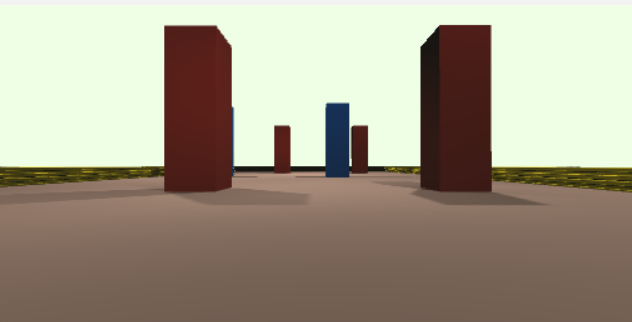
\includegraphics{Bilder/light_setting_standard.png}}\\
     \subfigure[reduced lighting]{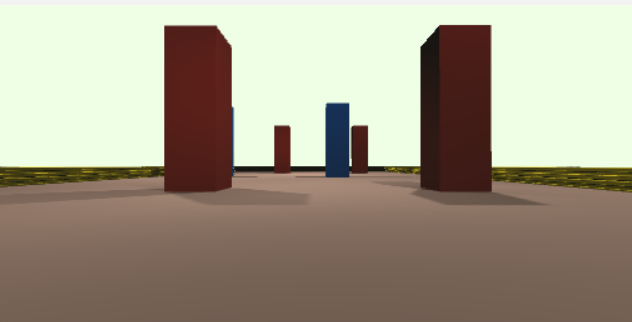
\includegraphics{Bilder/light_setting_reduced_lighting.png}}
     \subfigure[Increased lighting]{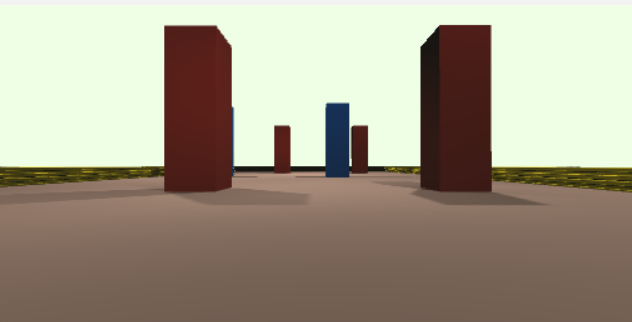
\includegraphics{Bilder/light_setting_increased_lighting.png}}
     \caption{different lightings TODO fix the images}
     \label{fig:3tracks}
\end{figure}

% TODO do we need an image equalization if the network is trained on varying light conditions?

\subsection*{Data Augmentation}
Convolutional Neural Networks require a lot of data to learn and generalize. Data augmentation is a technique to increase the amount of data available during training by applying transformations to the collected data. Collected data can be used to produce many more training examples by applying transformations such as rotation, translation, scaling, flipping and colour changes. In addition to providing a more diverse set of training data, this saves a lot of time since the new data points are not collected in simulation. \autocite{conditional_imitation_learning} employed a diverse set of data augmentation for their imitation learning approach that used a CNN.
During the training process the collected images will be augmented by applying random transformations to them. The transformations change the image similarly to how different environment conditions (e.g. lighting, camera quality and fog) might change the image. It is not yet decided which transformations will be used, possible candidates are changes in contrast, brightness and tone, as well as filters like Gaussian blur, Gaussian noise, salt-and-pepper noise.
Geometric transformations such as translations and rotations are not used since our control commands are not invariant to these transformations.


\begin{figure}
     \centering
     \subfigure[Original image]{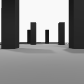
\includegraphics{Bilder/data_entry_original.png}}\\
     \subfigure[Gaussian Noise Mean 0 Sigma 5]{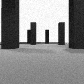
\includegraphics{Bilder/data_entry_augmented_gaussian_sigma_5.png}}\\
     \subfigure[salt-and-pepper noise]{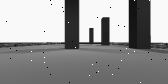
\includegraphics{Bilder/data_entry_augmented_salt_and_pepper.png}}
     \caption{Data augmentation examples}
     \label{fig:3tracks}
\end{figure}

% TODO find another paper with data augmentaton

\chapter{Evaluation and Experimentation}
%\label{cha:Experiments and Evaluation}
%\lipsum \autocite{DBLP:books/sp/HarderR01}

\section{Evaluation Metrics}

During the training and the final experiments, the agents are evaluated using the success rate, the average time needed to complete the map and the collision rate. The success rate is the percentage of episodes in which the agent successfully completed the map. These metrics were already used by \autocite{maximilian} and measure the most important properties of the agent's behaviour.

There will be additional metrics monitored during the training process to identify weak-points of the agent and erroneous behaviour. Monitoring the training process can provide insights into the agent's behaviour and help with choosing appropriate hyperparameters. TensorBoard will be used to visualize the monitored metrics.
These metrics could be the average cumulative reward, the average number of passed goals, the average distance travelled, the average amount of collisions, the average game duration and the average speed of the agent.

\section{Experiments}

The proposed experiments build on the scenarios from \autocite{maximilian}. These experiments included three parcours with different difficulty levels \ref{fig:3tracks} and conducted 3 different experiments with each trained agent. The first experiment used the same settings as the simulation environment. The second experiment was conducted under different lighting settings. The third one changed the motor power of the agent's two front wheels. All experiemnts primarily used the success rate to evaluate the agent's performance, the success rate is the proportion of succesfully completed parcours.

The first two experiments will be used in this thesis as well, using the same experiments allows for an easy comparison to the previous research. The experiment with varying motor power will be omitted since it is not related to the research goals of this thesis.




\subsection{Research Question 1 - Is it possible to train an autonomous driving agent consisting of a convolutional neural network with end-to-end reinforcement learning to reliably solve the parcours of all difficulty levels?}

The experiments under minimal changes will be used to judge if the agent is able to reliably solve all parcours. \ref{fig:3tracks} shows three parcours of different difficulty levels, there are further variations of these parours that change the positioning and color of the obstacles. The parcours are evaluated using the success rate, if the agent is able to reliably solve all parcours the agent and training implementation can be considered successful.

\begin{figure}
    \centering
    \subfigure[Easy]{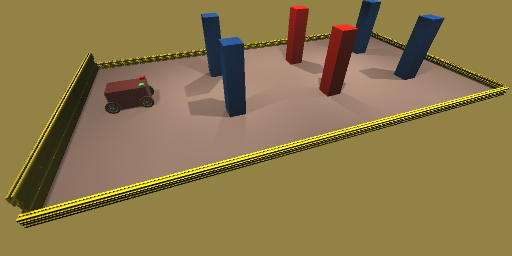
\includegraphics[width=0.3\textwidth]{Bilder/evaluation_easy.png}}\qquad
    \subfigure[Medium]{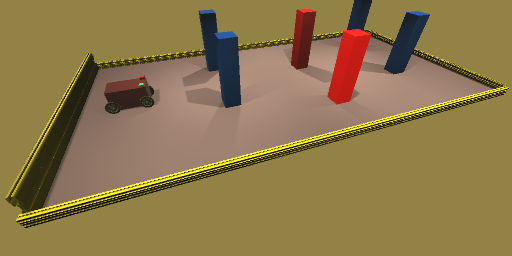
\includegraphics[width=0.3\textwidth]{Bilder/evaluation_medium.png}}\qquad
    \subfigure[Hard]{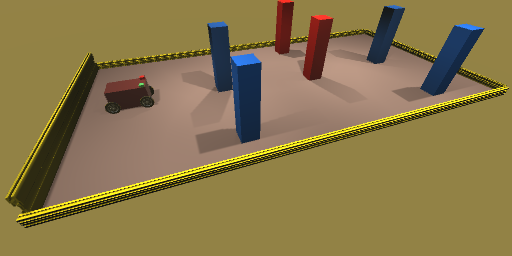
\includegraphics[width=0.3\textwidth]{Bilder/evaluation_hard.png}}\qquad
    \caption{Evaluation Tracks of different difficulties}
    \label{fig:3tracks}
\end{figure}

\subsection{Research Question 2 - Is it possible to use an end-to-end trained CNN to make the agent robust to changing light conditions?}

The evaluation parcours will be used with varying lighting settings to evaluate the agent's robustness towards changing light conditions. The agent's performance will be measured using the success rate, if the agent's performance is similar for all lighting settings the agent can be considered robust to changing light conditions.

\begin{figure}
    \centering
    \subfigure[Standard Lighting Agent POV]{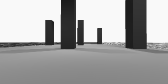
\includegraphics[width=0.3\textwidth]{Bilder/light_setting_pov_standard.png}}\qquad
    \subfigure[Standard Lighting Arena]{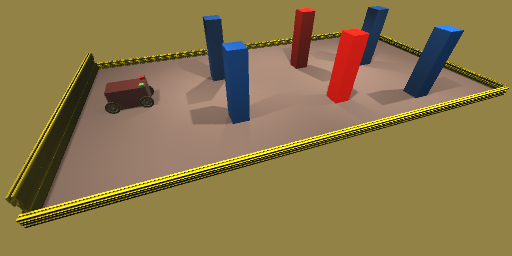
\includegraphics[width=0.4\textwidth]{Bilder/light_setting_arena_standard.png}}
    \subfigure[Reduced Lighting Agent POV]{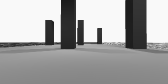
\includegraphics[width=0.3\textwidth]{Bilder/light_setting_pov_reduced_lighting.png}}\qquad
    \subfigure[Reduced Lighting Arena]{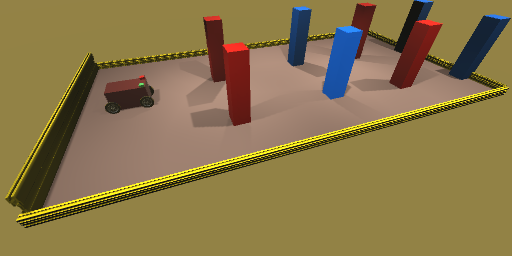
\includegraphics[width=0.4\textwidth]{Bilder/light_setting_arena_reduced_lighting.png}}
    \subfigure[Increased Lighting Agent POV]{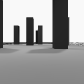
\includegraphics[width=0.3\textwidth]{Bilder/light_setting_pov_increased_lighting.png}}\qquad
    \subfigure[Increased Lighting Arena]{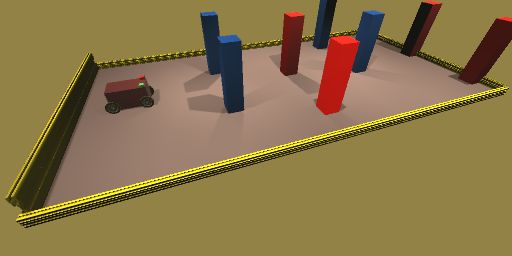
\includegraphics[width=0.4\textwidth]{Bilder/light_setting_arena_increased_lighting.png}}

    \caption{Agent Camera POV and Arena Screenshots of the different light settings} 
    \label{fig:light_settings}
\end{figure}

\subsection{Research Question 3 - Is it possible to use a neural network that can be transfered to a physical robot?}

To answer question 3 the developed agent will be evaluated on the JetBot's processing unit. There will be no physical experiments with the JetBot due to time constraints. Instead an evaluation parcour replay is generated in Python, the replay is then processed on the JetBot to measure its processing capabilities. The replay will consist of input-output pairs and metadata such as processing times. If the JetBot is able to reproduce the behaviour from the replay at sufficient speed, the agent can be considered transferable to the JetBot.

% kann ich die Experimente mit varying motor power weglassen?
% die Experimente stehen nicht so stark im Zusammenhang mit den beiden Research goals
% ja

\chapter{Schedule}
\label{cha:Schedule}


\begin{itemize}
    \item 1 month - Literature research: Search for further approaches to increasing light setting robustness and CNN training. 
    \item 2.5 months - Implementation of the training algorithm. Including preliminary testing/evaluation of configs and hyperparameters.
    \item 1 month - Training and Evaluation
    \item 1.5 months - Writing the thesis
\end{itemize}


exposetest

\printbibliography

% \setcounter{page}{122}
% \pagenumbering{gobble}
% %\pagenumbering{gobble}
\addchap{Erklärung}
Ich versichere, dass ich die vorliegende Arbeit mit dem Thema:

\begin{center}
\textit{\glqq\titel\grqq}\\[1em]
\end{center}
			
selbständig und nur unter Verwendung der angegebenen Quellen und Hilfsmittel angefertigt habe, insbesondere sind wörtliche oder sinngemäße Zitate als solche gekennzeichnet. Mir ist bekannt, dass Zuwiderhandlung auch nachträglich zur Aberkennung des Abschlusses führen kann. Ich versichere, dass das elektronische Exemplar mit den gedruckten Exemplaren übereinstimmt.
\par
\ort, den \eingereicht


\rule[-0.2cm]{5cm}{0.5pt}

\textsc{\autor} 
	% Selbständigkeitserklärung 

% Anhang -------------------------------------------------------------------
%		Die Inhalte des Anhangs werden analog zu den Kapiteln inkludiert.
%		Dies geschieht in der Datei Anhang.tex
% --------------------------------------------------------------------------
\appendix
\clearpage
\renewcommand*{\thesection}{\Alph{section}} 
\pagenumbering{Roman}
%\include{Inhalt/Anhang}



% Index --------------------------------------------------------------------
%		Zum Erstellen eines Index, die folgende Zeile auskommentieren.
% --------------------------------------------------------------------------
%\printindex		% Index hier einfügen
%\ofoot{}
%\include{Inhalt/Thesen}	% Thesen 

\end{document}
